%%%%%%%%%%%%%%%%%%%%%%%%%%%%%%%%%%%%%%%%%
% Structured General Purpose Assignment
% LaTeX Template
%
% This template has been downloaded from:
% http://www.latextemplates.com
%
% Original author:
% Ted Pavlic (http://www.tedpavlic.com)
%
% Note:
% The \lipsum[#] commands throughout this template generate dummy text
% to fill the template out. These commands should all be removed when 
% writing assignment content.
%
%%%%%%%%%%%%%%%%%%%%%%%%%%%%%%%%%%%%%%%%%

%----------------------------------------------------------------------------------------
%	PACKAGES AND OTHER DOCUMENT CONFIGURATIONS
%----------------------------------------------------------------------------------------

\documentclass{article}

\usepackage{fancyhdr} % Required for custom headers
\usepackage{lastpage} % Required to determine the last page for the footer
\usepackage{extramarks} % Required for headers and footers
\usepackage{graphicx} % Required to insert images
\usepackage{lipsum} % Used for inserting dummy 'Lorem ipsum' text into the template

% Margins
\topmargin=-0.45in
\evensidemargin=0in
\oddsidemargin=0in
\textwidth=6.5in
\textheight=9.0in
\headsep=0.25in 

\linespread{1.1} % Line spacing

% Set up the header and footer
\pagestyle{fancy}
\lhead{\hmwkAuthorName} % Top left header
\chead{\hmwkClass\ (\hmwkClassInstructor\ \hmwkClassTime): \hmwkTitle} % Top center header
\rhead{\firstxmark} % Top right header
\lfoot{\lastxmark} % Bottom left footer
\cfoot{} % Bottom center footer
\rfoot{Page\ \thepage\ of\ \pageref{LastPage}} % Bottom right footer
\renewcommand\headrulewidth{0.4pt} % Size of the header rule
\renewcommand\footrulewidth{0.4pt} % Size of the footer rule

\setlength\parindent{0pt} % Removes all indentation from paragraphs

%----------------------------------------------------------------------------------------
%	DOCUMENT STRUCTURE COMMANDS
%	Skip this unless you know what you're doing
%----------------------------------------------------------------------------------------

% Header and footer for when a page split occurs within a problem environment
\newcommand{\enterProblemHeader}[1]{
\nobreak\extramarks{#1}{#1 continued on next page\ldots}\nobreak
\nobreak\extramarks{#1 (continued)}{#1 continued on next page\ldots}\nobreak
}

% Header and footer for when a page split occurs between problem environments
\newcommand{\exitProblemHeader}[1]{
\nobreak\extramarks{#1 (continued)}{#1 continued on next page\ldots}\nobreak
\nobreak\extramarks{#1}{}\nobreak
}

\setcounter{secnumdepth}{0} % Removes default section numbers
\newcounter{homeworkProblemCounter} % Creates a counter to keep track of the number of problems

\newcommand{\homeworkProblemName}{}
\newenvironment{homeworkProblem}[1][Problem \arabic{homeworkProblemCounter}]{ % Makes a new environment called homeworkProblem which takes 1 argument (custom name) but the default is "Problem #"
\stepcounter{homeworkProblemCounter} % Increase counter for number of problems
\renewcommand{\homeworkProblemName}{#1} % Assign \homeworkProblemName the name of the problem
\section{\homeworkProblemName} % Make a section in the document with the custom problem count
\enterProblemHeader{\homeworkProblemName} % Header and footer within the environment
}{
\exitProblemHeader{\homeworkProblemName} % Header and footer after the environment
}

\newcommand{\problemAnswer}[1]{ % Defines the problem answer command with the content as the only argument
\noindent\framebox[\columnwidth][c]{\begin{minipage}{0.98\columnwidth}#1\end{minipage}} % Makes the box around the problem answer and puts the content inside
}

\newcommand{\homeworkSectionName}{}
\newenvironment{homeworkSection}[1]{ % New environment for sections within homework problems, takes 1 argument - the name of the section
\renewcommand{\homeworkSectionName}{#1} % Assign \homeworkSectionName to the name of the section from the environment argument
\subsection{\homeworkSectionName} % Make a subsection with the custom name of the subsection
\enterProblemHeader{\homeworkProblemName\ [\homeworkSectionName]} % Header and footer within the environment
}{
\enterProblemHeader{\homeworkProblemName} % Header and footer after the environment
}
   
%----------------------------------------------------------------------------------------
%	NAME AND CLASS SECTION
%----------------------------------------------------------------------------------------

\newcommand{\hmwkTitle}{Assignment\ \#2} % Assignment title
\newcommand{\hmwkDueDate}{Monday,\ March\ 9,\ 2015} % Due date
\newcommand{\hmwkClass}{CS\ 280} % Course/class
\newcommand{\hmwkClassTime}{9:30am} % Class/lecture time
\newcommand{\hmwkClassInstructor}{Malik} % Teacher/lecturer
\newcommand{\hmwkAuthorName}{Alex Hall and Rachel Albert} % Your name

%----------------------------------------------------------------------------------------
%	TITLE PAGE
%----------------------------------------------------------------------------------------

\title{
\vspace{2in}
\textmd{\textbf{\hmwkClass:\ \hmwkTitle}}\\
\normalsize\vspace{0.1in}\small{Due\ on\ \hmwkDueDate}\\
\vspace{0.1in}\large{\textit{\hmwkClassInstructor\ \hmwkClassTime}}
\vspace{3in}
}

\author{\textbf{\hmwkAuthorName}}
\date{} % Insert date here if you want it to appear below your name

%----------------------------------------------------------------------------------------

\begin{document}

%\maketitle

%----------------------------------------------------------------------------------------
%	TABLE OF CONTENTS
%----------------------------------------------------------------------------------------

%\setcounter{tocdepth}{1} % Uncomment this line if you don't want subsections listed in the ToC

%\newpage
%\tableofcontents
%\newpage

%----------------------------------------------------------------------------------------
%	PROBLEM 1
%----------------------------------------------------------------------------------------

% To have just one problem per page, simply put a \clearpage after each problem

\begin{homeworkProblem}
\begin{homeworkSection}{(1.1)} % Section within problem
\vspace{10pt}
	
	(a) As a warm-up, use the raw pixels as features to train a linear svm. Plot the error rate vs the number of training examples.
	\newline
	
	\problemAnswer{ % Answer
	
	Here we plot the accuracy vs. number of training examples for raw pixel features.
	
	\begin{center}
	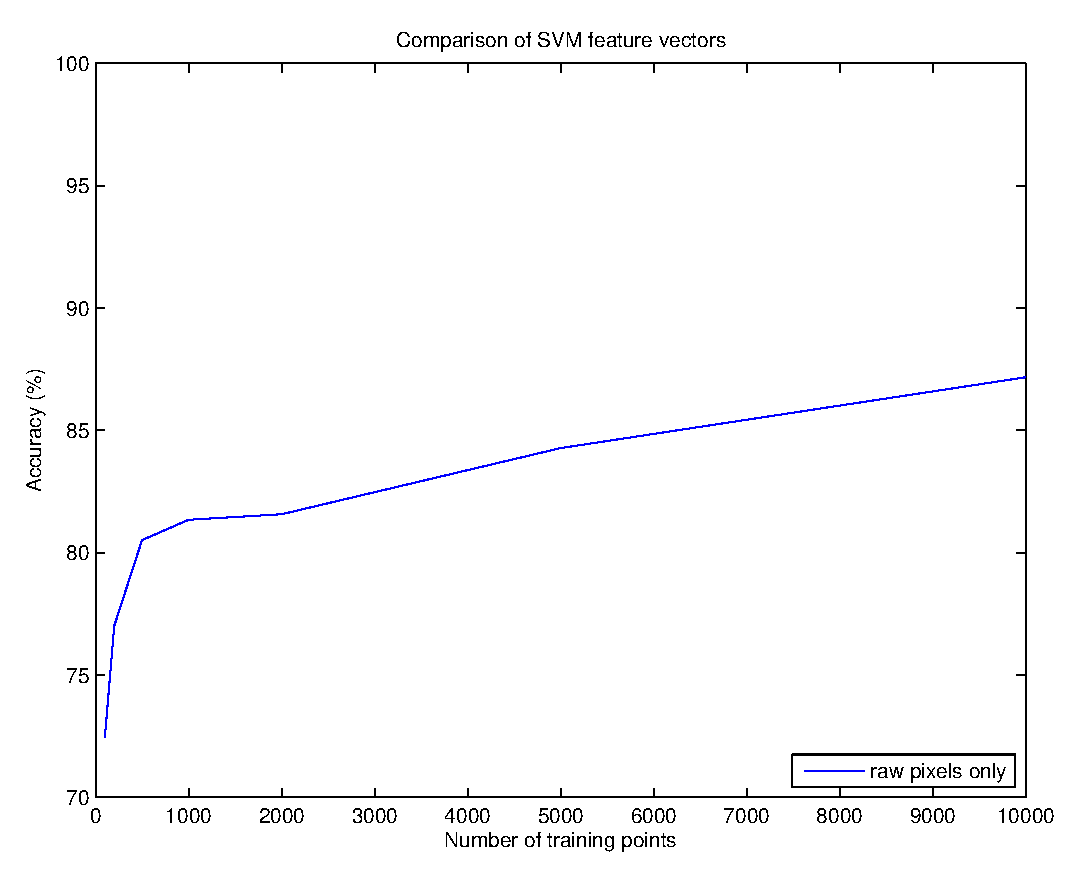
\includegraphics[width=0.75\columnwidth]{pixOnly} % Example image
	\end{center}
	}
\end{homeworkSection}

\begin{homeworkSection}{(1.2)} % Section within problem
\vspace{10pt}

	(a) Explain briefly why adding these features should help over raw pixel values.
	\newline
	
	\problemAnswer{ 
	
	The local sums provide more information about larger neighborhoods in the image, which equates to more relational information. The overlapping windows provide some translational invariance.
	
	}
	
	(b) Implement these features and use them to train a linear svm. Plot the error rate vs the number of
	training examples. Do you get a significant boost over Q1?
	\newline
	
	\problemAnswer{ 
	
	Here we plot the error rate vs. number of training examples for both raw pixel features alone (in Blue) and raw pixel features plus local cxc neighborhood sums with overlapping windows of size c/2 for c=4,7 (in Green). For a small number of training examples our performance is better with the additional features than for the raw pixel features alone. However, with more training examples the raw pixels surpasses the raw pixels plus the pyramid features.
	
	\begin{center}
	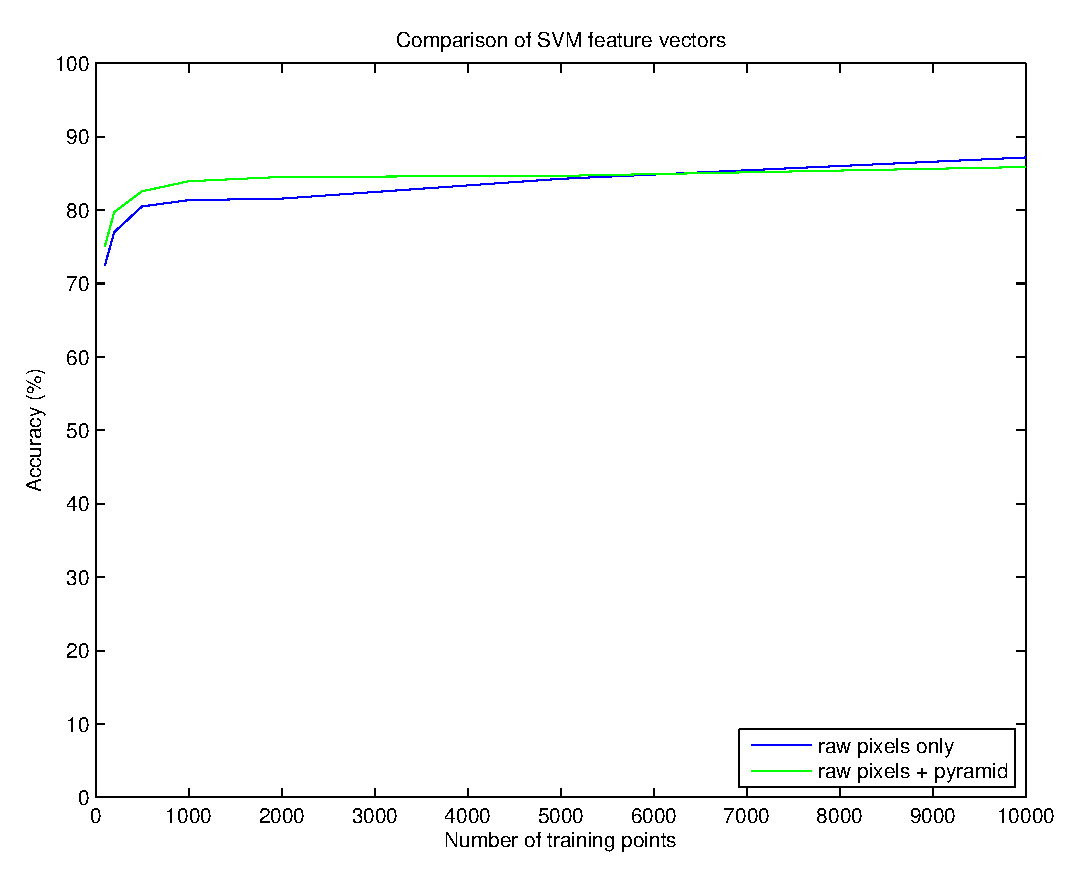
\includegraphics[width=0.75\columnwidth]{pixAndPyr} % Example image
	\end{center}
	
	}

\end{homeworkSection}

\begin{homeworkSection}{(1.3)} % Section within problem
\vspace{10pt}

	(a) Explain briefly why gradient orientations should help over pixel intensities : what is the gradient orientation trying to capture?
	\newline
	
	\problemAnswer{ 
	
	ANSWER GOES HERE
	
	}
	
	(b) Implement these features and use them to train a linear SVM. For computing the gradient, use the tap filter:[?1 0 1]. Use 9 orientation bins. Use the same cell sizes (4 and 7) as in Q2. Plot the error rate vs the number of training examples. Do you get a significant boost over Q2?
	\newline
	
	\problemAnswer{ 
	
	ANSWER GOES HERE
	
	\begin{center}
	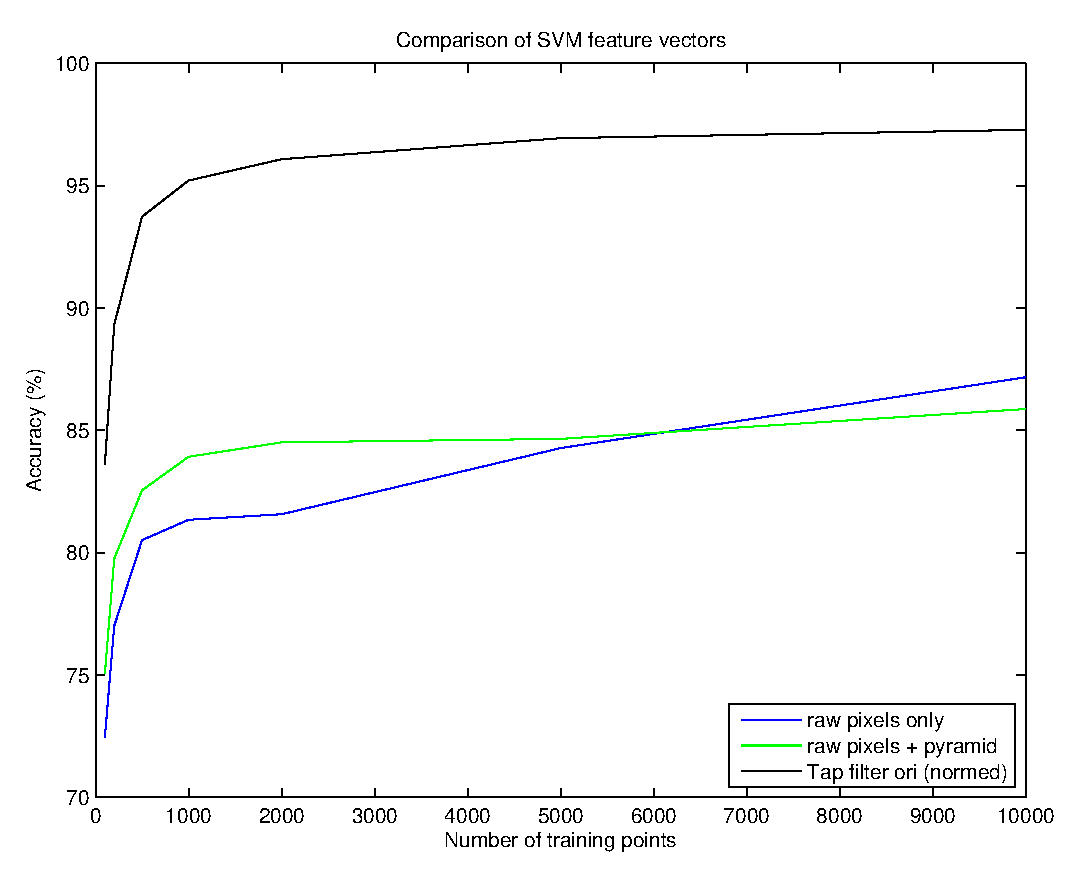
\includegraphics[width=0.75\columnwidth]{normedTap} % Example image
	\end{center}
	
	}
	
	(c) Does the performance drop if you don�t normalize the histograms before concatenating them? Why or why not? Plot error rate vs the number of training examples.
	\newline
	
	\problemAnswer{ 
	
	ANSWER GOES HERE
	
	\begin{center}
	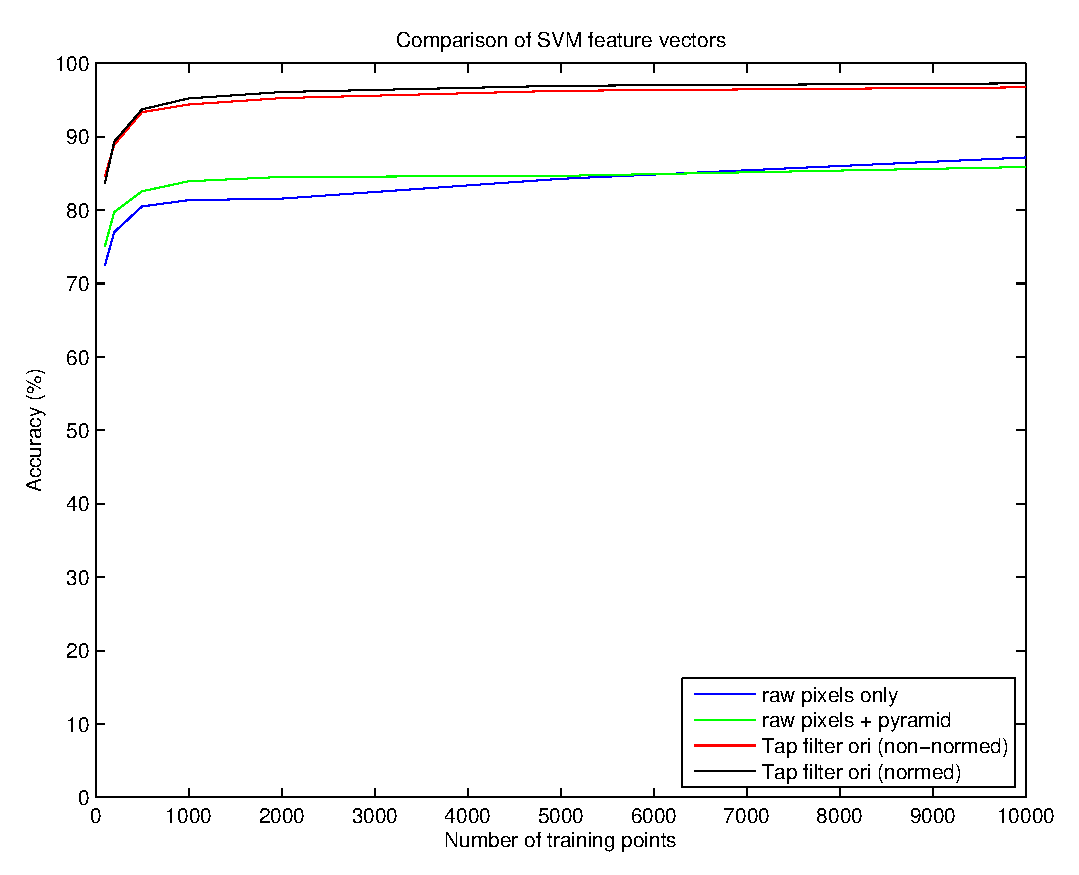
\includegraphics[width=0.75\columnwidth]{nonNormedTap} % Example image
	\end{center}
	
	}
	
	(d) How does performance change if you replace the tap filter with a Gaussian derivative filter?
	\newline
	
	\problemAnswer{ 
	
	ANSWER GOES HERE
	
	\begin{center}
	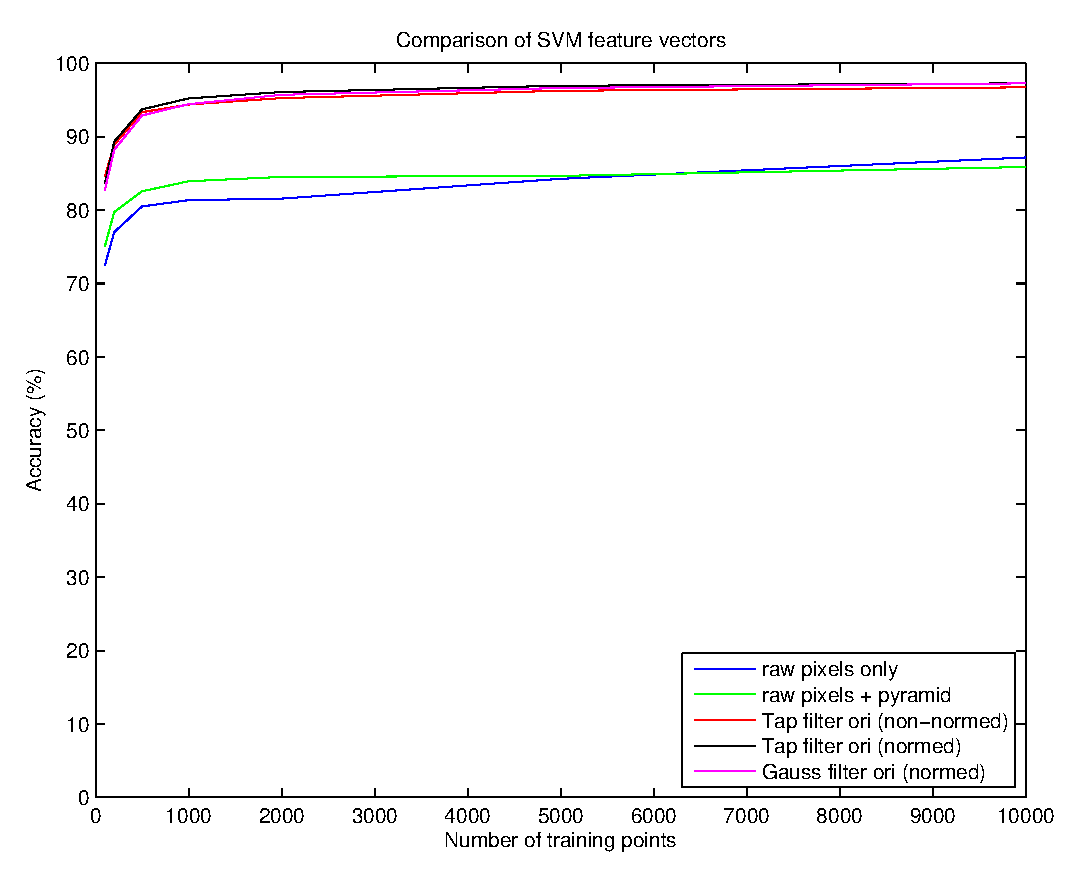
\includegraphics[width=0.75\columnwidth]{normedGauss} % Example image
	\end{center}
	
	}
	
	(e) Explain how you choose the hyper-parameter in linear SVM and why.
	\newline
	
	\problemAnswer{ 
	
	ANSWER GOES HERE
	
	}
\end{homeworkSection}
	
\begin{homeworkSection}{(1.4)} % Section within problem
\vspace{10pt}
	
	(a) Visualize the images on which you go wrong. Do the errors your classifier makes seem reasonable to you? How many of these images do you as a human have a hard time recognizing?
	\newline
	
	\problemAnswer{ 
	
	ANSWER GOES HERE
	
	}

\end{homeworkSection}

\end{homeworkProblem}

%----------------------------------------------------------------------------------------
%	PROBLEM 2
%----------------------------------------------------------------------------------------

\begin{homeworkProblem}
\begin{homeworkSection}{(2.1)} % Section within problem
\vspace{10pt}

	(1) Draw a schematic of the neural network architecture described above. Clearly label all the layers of the network (including the non-linearity).
	\newline
	
	\problemAnswer{ % Answer
	
	ANSWER GOES HERE (+FIGURE)
	
	}
	
	(2) Train this network for digit classification. Report the accuracy on the test set. How many parameters does this network have?
	
	\problemAnswer{ % Answer
	
	The accuracy for the two layer fully connected network is ???.
	The network has 20*784 parameters for ip1 and 500*20 parameters for ip2, for a total of 25680 parameters.
	
	}
	
	(3) Use three hidden layers of 20, 50 and 500 units respectively. Report the accuracy on the test set. How many parameters does this network have?
	
	\problemAnswer{ % Answer
	
	The accuracy for the three layer fully connected network is ???.
	The network has 20*784 parameters for ip1, plus 50*20 parameters for ip2, and 500*20 parameters for ip3, for a total of 25680000 parameters.
	
	}
	
	(4) Compare the performance of both these networks. Why is the performance greater/lower or the same?
	
	\problemAnswer{ % Answer
	
	ANSWER GOES HERE
	
	}
	(5) Change the non-linearity to Sigmoid and re-train the network. Do you observe any differences? If the depth of the network is increased - what effect would the Sigmoid non-linearity have on the magnitude of the gradients? Is this desirable? Is the behavior of ReLu units different?
	
	\problemAnswer{ % Answer
	
	ANSWER GOES HERE
	
	}

\end{homeworkSection}

\begin{homeworkSection}{(2.2)} % Section within problem
\vspace{10pt}

	(1) Report the performance of the LeNet architecture. How many parameters does this network have? Train the LeNet using only 10K examples and compare the performance with the SVM classifier you trained in the first part of the homework.
	\newline
	
	\problemAnswer{ % Answer
	
	The LeNet Architecture has 430500 parameters. The performance for 10K examples is 97.36\%, compared to 97.28\% correct for the normalized Tap filter SVM classifier.
	
	}
	
	(2) Both LeNet and FC network have 20, 50, 500 units in the three hidden layers. Considering this, compare the performance of LeNet with the Fully connected(FC) network with three hidden layers.
	
	\problemAnswer{ % Answer
	
	The LeNet network has a performance of 97.36\% compared to ??? for the three-layer FC network.
	
	}
	
	(3) Now, reduce the number of units in the third hidden layer of the LeNet to 32. Lets call this LeNet2. Compare the performance with the fully connected network. Why is the performance greater/lower or the same?
	
	\problemAnswer{ % Answer
	
	The performance of LeNet2 is 98.58\% compared to ??? for the three-layer FC network. EXPLANATION GOES HERE.
	
	}
	
	(4) Experiment with the kernel sizes in LeNet2. Try kernel sizes of 3 and 7. What do you find?
	
	\problemAnswer{ % Answer
	
	The performance of LeNet2 is 98.38\% and 98.53\% for kernel sizes of 3 and 7, respectively.
	
	}
	(5) Visualize the first layer filters of the original LeNet network. What do you find? Based on this visualization - can you comment on what computation first layer is performing?
	
	\problemAnswer{ % Answer
	
	Here is a visualization of the first layer filters (note: image size is very small).
			
%	\begin{center}
%	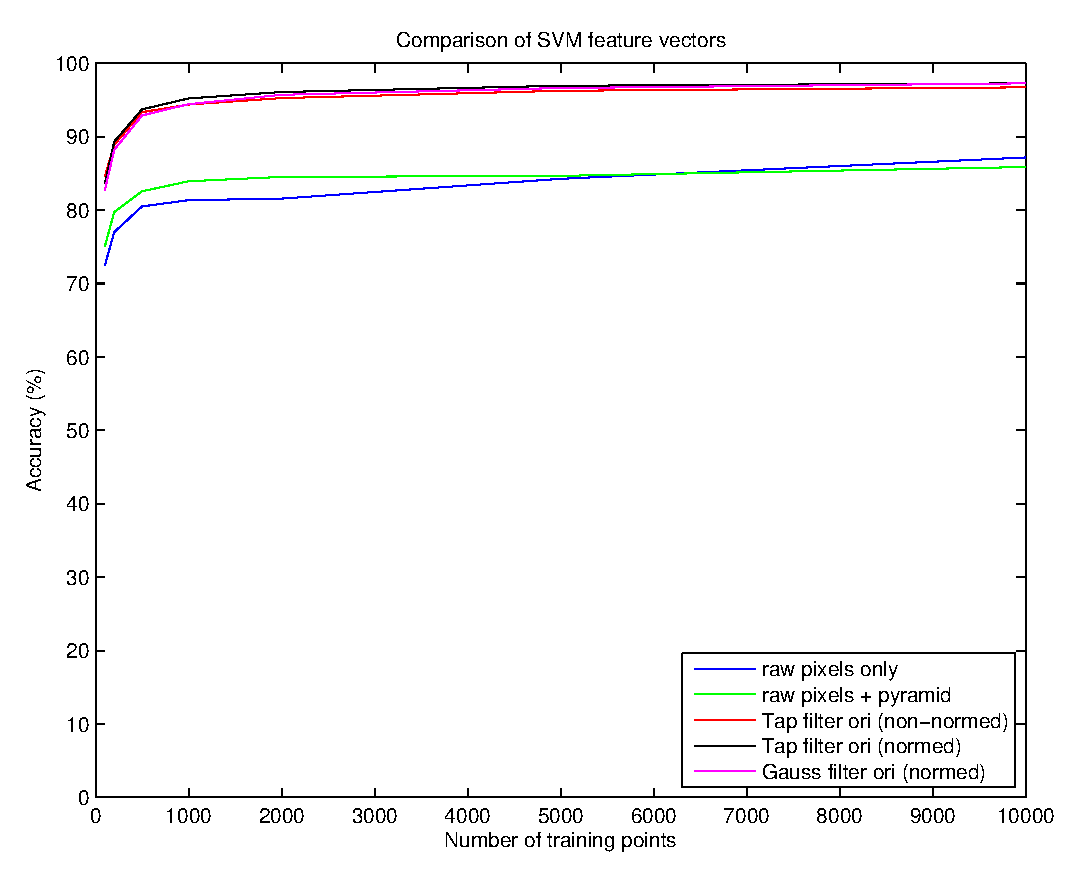
\includegraphics[width=0.75\columnwidth]{normedGauss} % Example image
%	\end{center}
	
	FURTHER EXPLANATION GOES HERE
	
	}
	(6) Based on your results, list the pros and cons of using a FC network in comparison to the ConvNet. Is the ConvNet more scalable to larger images? If yes, why and if no, why not?
	
	\problemAnswer{ % Answer
	
	ANSWER GOES HERE
	
	}

\end{homeworkSection}

\end{homeworkProblem}

\end{document}
